\chapter{System Design}

In this chapter the project is further analysed. Diagrams are given
and other notions are described, setting up the premises for implementing
the OSname based on the ARINC 653 standard.
\todo[inline, color=green]{define an OS name somewhere to be used throughout
the report}
\section{System Overview}
As a means to both explaining the system and as a practical development
model, the system can be thought of as being made up of layers.
Each layer being an abstraction of workings in the layers beneath it,
with the partitions at the top and the hardware at the bottom.
The model in \ref{fig:simple_system} is defined by the ARINC 653 standard
and expanded upon here with drivers being build on top of the HAL library,
instead of directly on top of the hardware, creating an extra layer of
 abstraction.

\begin{labeling}{HAL and CMSIS}
	\item [\textbf{Partitions}]
		independent program units that contain applications. These
		applications can in turn interact with other systems. The
		partitions are achieving this in complete isolation from 
		one another.
	\item [\textbf{APEX}]
		defines the methods by which the partitions talk to other 
		modules and
		interact with other partitions or the OS, running
		on the same core module or connected to other ARINC systems.
	\item [\textbf{OS}]
		provides the infrastructure for partitions to operate. This 
		includes their scheduling, message passing and processes 
		the APEX calls.
	\item [\textbf{XML}]
		contains the data necessary for the system initialisation.
	\item [\textbf{Drivers}]
		define the way the hardware should run.	
		They serve the OS with methods to create an environment in which
		partitions can be run and scheduled without influencing one
		another.
	\item [\textbf{HAL and CMSIS}]
		are libraries that provide hardware abstraction layers for
		setting up the hardware. 
	\item [\textbf{Hardware}]
		the physical platform on which the OS is run. This 
		includes the CPU and its peripherals.
\end{labeling}

\begin{figure}[H]
\centering
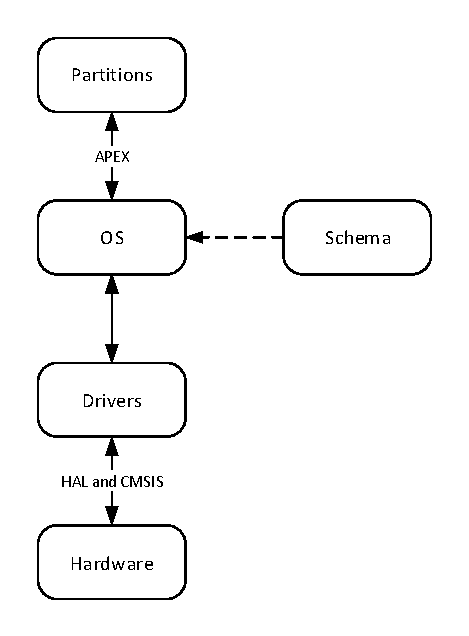
\includegraphics[width=7cm,keepaspectratio]{simple_system_architecture.pdf}
\captionof{figure}{A simple system overview}
\label{fig:simple_system}
\end{figure}

In the rest of the chapter the different layers are described,
from bottom up, 
together with their core components.The hardware specifications
are outlined, as well as explaining how the rest of the system is
set up.


\section{Hardware}

As mentioned in the \nameref{section:settleing_platform} section,
the hardware used for the development of this system is the Mini-M4
board. It is build around the STM32F415RG microcontroller, based on
an ARM Cortex-M4 core. This is a 32-bit RISC architecture CPU using 
the ARM intruction set \cite{arm_architecture}. Additional information
was found in the ARM technical reference \cite{arm_technical} 

The chip provides two interfaces for debugging:
%page 1683 reference manual
\begin{itemize}[noitemsep]
	\item JTAG Debug Port (JTAG-DP)
	\item Serial Wire Debug Port (SW-DP)
\end{itemize}
There was no thought process involved in choosing one of the two.
The JTAG interface is enabled by default, and worked right from the
early phases of the project. In some situations, SW would have been
preferred to JTAG, due to space(2 pins instead of 5) constraints
 or the IDE used.

JTAG is actually an association that develops standards about how 
physical circuit boards should be tested. However, for the rest of
the document, JTAG will be referred to as the main communication interface
to the Mini-M4 board. This will mainly be used for flashing the program
on the chip and debugging it. In order for a computer to access this
interface, there is need the STLINK-V2, that would 
use the USB as a mean to communicate with the JTAG port on the chip.

Another way of communicating to the chip is the serial communication.
For this purpose the UART will be used. This is common peripheral for 
embedded devices, and it needs to be set up before it can be used. This
involves initialising the UART, configuring the data format and the
transmission speed and sending the actual data. In order to see this data
on a computer, one could use an USB-to-serial adapter. This would then
create a vitual COM (Communication port), that could be accessed using
a serial console such as PuTTY.
\\\\
The Mini-M4 board would have to accommodate the 5 wires from the JTAG,
the 2 wires from the UART, and to receive power through the built-in
mini USB port, in order to be ready for the development process.

\section{Memory Map}
\label{sec:memory_map}
The STM32F415RG microcontroller has 1 MB of flash memory. The flash 
is non-volatile memory, used for storing programs and
data.

There are 192 KB of RAM, divided into 128 KB of SRAM and 64 KB of 
CCM data RAM.
The SRAM is volatile memory, where the 'static' tag means 
that it does not need to be refreshed in order to
keep its state. This is divided furthermore into a section of 112 KB, and 
another of 16 KB, which can be useful if one needs to boot from RAM. Anyway, these are adjacent in address space and can be treated as 
one block. (REFERENCE)
The memory has a feature called bit-banding, in order to let the system
to perform atomical operations on bits.
%https://spin.atomicobject.com/2013/02/08/bit-banding/
%http://infocenter.arm.com/help/index.jsp?topic=/com.arm.doc.dai0179b/CHDJHIDF.html

The other 64 KB of CCM data RAM are always ready for access by the CPU,
but cannot be accessed by the peripherals through direct memory access.
Beside the 192 KB of SRAM, there are 4 KB of SRAM used for backup purposes.
These won't be used, since they not represent the scope of the project.
%http://hackaday.com/2012/11/15/in-depth-comparison-at-stm32-f3-and-f4-discovery-boards/
%http://electronics.stackexchange.com/questions/27550/what-is-bit-banding
%http://libopencm3.org/wiki/Run_From_RAM
%stm32f4415 pag 74 figure 18

Figure \ref{fig:memory_model} represents a simplified model of the 
memory map implemented in the STM32F415RG microcontroller. The blocks
on the left column are legacy of the ARM Architecture. This provides 
4 GB of addressable memory in all.
These regions are correlated to the microcontroller\textquotesingle s
actual memory, as it can be seen in the right column. Each block in this
column contain their start and end addresses, on their side.
\begin{figure}[H]
\centering
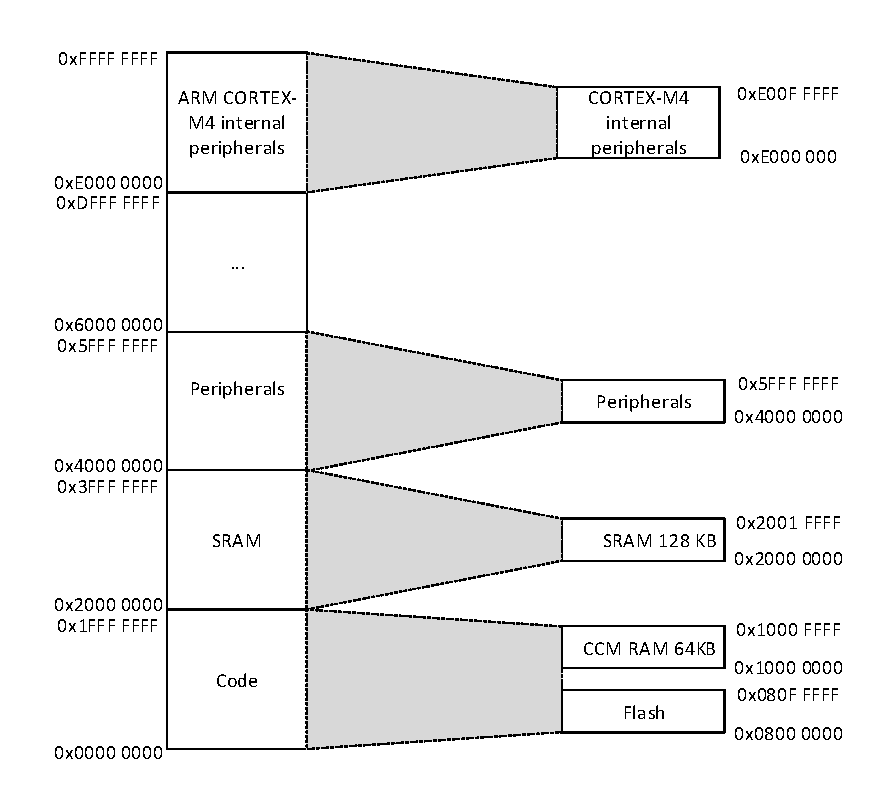
\includegraphics[width=\linewidth,keepaspectratio]{memory_model.pdf}
\captionof{figure}{The memory map (inspired by: 
REFERENCE PAGE 74)}
\label{fig:memory_model}
\end{figure}
\todo{REFERENCE PAGE 74}

The input/output are mapped as well in the memory. This can be seen in
the upper two blocks of the memory map, where there are the 
microcontroller\textquotesingle s peripherals, as well as the Cortex-M4
specifics.

\section{HAL and CMSIS}
These two libraries are truly the workhorse when dealing with the 
board\textquotesingle s peripherals. By using them, the development
process usually has a quick start, removing the steepness of the 
learning curve.	\\
HAL stands for Hardware Abstraction layer and is provided by the chip manufacturer - STMicroelectronics. The source files are available at
their website, along with its documentation \cite{HAL_library}.
The CMSIS (Cortex Microcontroller Software Interface Standard)
can be seen more as a framework, than a library
 \cite{CMSIS_core_library}. It is provided
by ARM, the company that developed the chip architecture.

As seen in figure \ref{fig:CMSIS_HAL}, CMSIS
is defining the data structures and address mapping of all peripherals.
Besides this, it can be used to configure the microcontroller
oscillators, ad well as providing support for the instrumentation trace during debug sessions \cite{cmsis_reference}.
The HAL library can then use these definitions for implementing its
utilities. One could easily say that HAL is build on top of CMSIS.
This can be further understood by looking at the way CMSIS handles
the exceptions occurring in the chip, while the HAL library configures
these interrupts.

 
\begin{figure}[H]
\centering
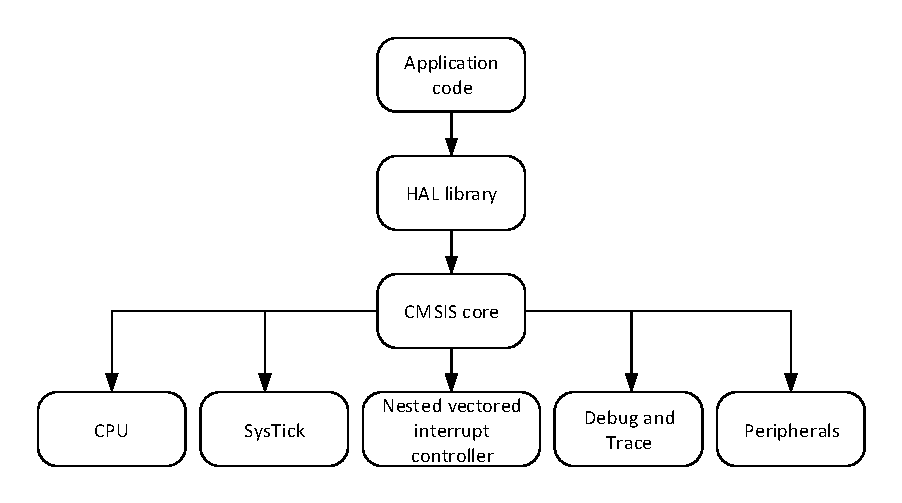
\includegraphics[width=\linewidth,keepaspectratio]{HAL_CMSIS.pdf}
\captionof{figure}{The structure of the libraries (inspired by: 
\cite{cmsis_picture})}
\label{fig:CMSIS_HAL}
\end{figure}

\section{Drivers}

The drivers controlling the hardware would have to be implemented at an 
early stage of the project, in order to have access to the low level
subsystems.
The following list contains the drivers that would provide the OS a basic
interface to access the hardware.

\begin{labeling}{Watchdog timer}
	\item [\textbf{UART}] used by the system to communicate with the outside
	world. This can either receive or transmit data to another UART device
	\item [\textbf{Watchdog timer}] necessary to ensure recovery
	in case of a hardware fault or program error. If this happens, the
	program would be restarted from a safe state
	\item [\textbf{System Clock}] provide the frequency at which the
	peripherals are synchronised. This can be later on scaled up or down
	to generate the CPU\textquotesingle s and peripherals\textquotesingle
	clock.
	The system clock relies on an oscillator.
	There is a multitude of choices, ranging from internal or external
	oscillators, to high or low speed crystals. In some cases, certain
	peripherals can use their own, independent clock sources that also have
	to be configured
	\item [\textbf{MPU}] provides the system a way to manage its
	memory. This is required by the ARINC 653 standard. 
	Operating systems built on more advanced processors generally use 
	an MMU
	\item [\textbf{RTC}] has purpose of this is to keep track of 
	time accurately. Usually it uses  a 32,768kHz oscillator as a 
	clock source, which is the standard in the field
	\item [\textbf{Timing}] has the purpose of keep track of 
	relative time. As the standard specifies, it should be counting 
	nanoseconds
	\item [\textbf{Delay}] is a simple function, based on a calling another
	function from the HAL library. It delays the execution 
	of the program by a factor of milliseconds. Mainly used in debugging
	\item [\textbf{LEDs}] mainly used for debugging. They are
	are connected to two of the GPIO pins
\end{labeling}

These drivers should be implemented as standalone .c files. They could then
be used by including their header files where needed and calling their
functions.
The basic functionalities of a driver are:
\begin{itemize}[noitemsep]
	\item initialisation of the peripheral
	\item usage of its resources
	\item de initialisation (if needed) \todo {spelling}
\end{itemize}

\section{OS}
\subsection{Scheduler}
\todo {line formatting, add some returns}
A scheduler decides which process should be executed by the processor available, according to some rules. In this implementation we have 2 levels of scheduling, one to switch between partitions and a second one for processing the processes of each partition.

For the first one we used a Manual Scheduler, that gives a certain amount of time of processor to each partition, according to its demand and importance. Those values can't be changed in running time, following the same rules during the whole execution. Every milisecond we verify if the time of the partition running has reached the timeout, if so, we switch the context for the next partition. And the new partition gets the processor.

The second one is a Pre-emptive Priority Scheduler, based on the processes' priority, in which is executed the one with the highest priority until it loses the processor to other partition. Every milisecond we pick the process, from the array of processes of that partition, with the highest priority and run in the processor.

\subsubsection{Context switching}
Context switching is to switch from executing one block of code $b_1$ to another block of code $b_2$
with the intend to eventually return to $b_1$ in a way that is transparent to the blocks of code.
This allows for code to be partitioned into separate independent blocks that can run concurrently.
This is opposed to monolithic blocks of code that entirely control the flow of execution.
Therefore, context switching is essential for any operating system that wishes to utilise a scheduler to allow concurrent execution of code.
Context switching works by saving the state of the CPU registers from one context to memory,
and then switching to another context by restoring the state of the registers previously saved in memory.
Since context switching must manipulate registers directly and individually, it is a feature that must be implemented
on a very low level of abstraction, and it can change significantly from one CPU architecture to another.
The scope of this project is to only implement an operating system for a Cortex M4. Hence context switching needs only
to work on the architecture used by this chip.\\
Context Switching on the Cortex M4 is partially handled by the Nested Vectored Interrupt Controller (NVIC).
When an exception (this includes interrupts) occurs, the NVIC will change context to an exception handler.
Upon changing context from regular code to the exception handler, the NVIC will save the registers R0-R3, R12, LR, PC and PSR
on the stack. These are only some of the registers. Why the decision was made to make the hardware save some of the
registers instead of letting software handle all, is unknown. \todo{Research harder the reason why the NVIC saves some register.}
When the exception handling routine exits, and control is handed back to the NVIC,
the NVIC will restore these registers again.\\
If the operating system wishes to switch context, it must save the remaining registers, R4-R11, and the stack pointer to memory
pick a new context to restore, reload the registers R4-R11 and the stack pointer of the new context from memory,
and hand back control to the NVIC. The NVIC will then reload the remaining registers from the stack of the new context. To see a figure of the registers and who saves them, see figure \ref{tab:registers}\\\\


\begin{table}[H]
	\centering
	\begin{tabular}{|c|c|p{9.5cm}|}
		\hline
		Register	&	Saved by	&	Purpose\\
		\hline
		R0			&	Hardware	&	General purpose (Argument value + return value)\\
		\hline
		R1-R3		&	Hardware	&	General purpose (Argument value)\\
		\hline
		R4-R11		&	Software	&	General purpose (Local variable)\\
		\hline
		R12			&	Hardware	&	General purpose (Intra-Procedure-call scratch)\\
		\hline
		R13 (SP)	&	Software	&	Stack pointer [Banked]\\
		MSP			&	Software	&	Master stack pointer (Stack pointer for kernel space)\\
		PSP			&	Software	&	Process stack pointer (Stack pointer for user space)\\
		\hline
		R14 (LR)	&	Hardware	&	Link register\\
		\hline
		R15 (PC)	&	Hardware	&	Program Counter\\
		\hline
		xPSR		&	Hardware	& 	Special-purpose Program Status Register\\
		\hline
	\end{tabular}
	\captionof{table}{A table of the CPU registers of a Cortex M4. Notice that register R13 (stack pointer) is banked;
	there are separate registers for user space and kernel space.
	For registers, aliases are written in parenthesis, and for purpose, calling convention is written in parenthesis.}
	\label{tab:registers}
\end{table}
As added complexity, the Cortex M4 utilises two different stack pointers, the Master Stack Pointer (MSP) and the Process Stack Pointer (PSP).
The MSP is intended for kernel space execution and the PSP is intended for user space execution, but there is no enforcement.
Switching between the two cannot be done in an exception handler, but must instead be done by the NVIC.
Since the path to the new context goes through the NVIC, the NVIC is also partially responsible setting the state of the processor.
This is done by loading an EXC\_RETURN value into the Program Counter. See table \ref{tab:exc-return} for the different values.
To make context switching transparent to the applications running, it's important that the state the processor returns to, is the
same it earlier came from. Therefore, upon entry into the interrupt routine, the NVIC loads the appropriate EXC\_RETURN into the Link
register. This value must be saved by software to assure it can return to the right state.


\begin{table}[H]

	\centering
	\begin{tabular}{|c|p{10cm}|}
		\hline
		Value			&	Description 	\\
		\hline
		0xFFFF FFF1 	&	Return to Handler mode, using the Master Stack Pointer, but without the floating point unit.	\\
		\hline
		0xFFFF FFF9		&	Return to Thread mode, using the Master Stack Pointer, but without the floating point unit.		\\
		\hline
		0xFFFF FFFD		&	Return to Thread mode, using the Process Stack Pointer, but without the floating point unit.	\\
		\hline
		0xFFFF FFE1		&	Return to Handler mode, using the Master Stack Pointer, with the floating point unit.			\\
		\hline
		0xFFFF FFE9		&	Return to Thread mode, using the Master Stack Pointer, with the floating point unit.			\\
		\hline
		0xFFFF FFED		&	Return to Thread mode, using the Process Stack Pointer, with the floating point unit.			\\
		\hline
	\end{tabular}
	\captionof{table}{
		A table of the possible EXC\_RETURN values. An interrupt service routine
		 is exited by loading one of these values into the Program Counter register.	}
	\label{tab:exc-return}
\end{table}

\subsection{Interpartition communication}

\subsubsection{Queuing Ports}

\subsubsection{Sampling Ports}


\subsection{Memory Management}
ARINC 653 advertises time and space separation covered in.
\todo[inline]{ref to sec in analysis}
To accommodate for the feature of separating partitions in space,
this operating system relies on the memory management unit (MPU)
to manage permissions across sections of memory,
ensuring that partitions stay within a dedicated memory space.

\subsection{something about ARINC on memory management}
The ARINC 653 standard OS, uses a statically allocated memory layout for everything
that gets compiled.
\todo[inline]{reference to standard}
This means that no memory allocation is permitted at runtime
outside predefined memory sections.
This policy ensures a fixed and predictable sandboxing environment, where partitions
can not restrict other parts of the system by occupying memory resources.
It also gives the system developer a way to ensure that the system has enough memory
for all processes to function correctly, given that this amount can be predetermined.

Memory regions are declared in the XML file, included at compile time, for a list
of different system features, like individual partitions and communication buffers.
All of this information is important for different reasons when setting up the system.
The rest of this section will deal with the subject of managing memory regions on a STM32F415 chip
and categorizing and analysing the memory requirements into a single memory strategy to implement in
\todo[inline]{ref to memory management implementation}.

\subsection{the MPU on a STM32F415}



\subsection{memory strategy}
To allocate all the partitions in the most optimized way we try to have the less spare memory possible. As
 the biggest partitions are less likely to perfectly fit in a region, since the regions are power of 2,
  the biggest the power the biggest the jumps of size, we start by allocating them. Then, if there are
   empty subregions, we try to fit in the other partitions in the best combination possible, trying
    different possibilities with the non allocated ones. In case that a certain partition doesn't full
    fill the last subregion we update the partition size with that free space, so that empty space can be
    used by the partition too, instead of being empty always. That can also help to avoid some errors, 
    for example if the initial partition size wasn't enough.



\subsection{System calls}
To improve security and robustness, many modern operating systems make clear 
distinctions between the kernel and applications, and they restrict application
code from accessing certain periphrial hardware (e.g. storage devices, I/O
devices, etc.) as well as control registers of the CPU. 
To restrict only certain code from certain features requires hardware support.
To accomplish this, many modern CPUs contain two or more different execution
levels. Normally, the kernel will run in the most privileged execution level
while application code runs in a more restricted execution level. This prevents
application code from changing the state of any resources shared with other
application. This is critical to accomplish ARINC 653's strict space and time 
seperation. If partition level code is not run in an unprivileged mode, it will
be able to directly change the CPU time and memory space allocated to it. This
would negatively affect the partition the resources were stolen from. However,
since partition level code does on occation need access to some shared resources,
yet is unable to do so directly, it must request the kernel do it. To do this,
partition level code must preload the general purpose CPU registers, and if
necessary the stack, with a value to identify what the partition wishes the
kernel do, as well as call arguments, then generate an interrupt which will be
caught by the kernel. Based on the content of the general purpose CPU registers
and the stack, the kernel determines what the partition level code requested,
executes the necessary functions and returns the result in the general purpose 
CPU registers and the stack.


\section{XML}

\todo[inline, color=green]{TO BE MOVED: An XML file is provided by the system developer
 at compile time.It defines how the top layers interact and set the
  requirements of the drivers and the underlying hardware.
Every layer contains a list of components, which provides the
 functionalities of that layer.
Beneath graphical overview of the different layers with their core
 components is provided.}

\section{APEX}

\section{Partitions and processes}

\subsection{Partitions}

\subsection{Processes}

\subsection{Error Handling}

\section{Agile development}

\section{Discussion}

Figure \ref{fig:advanced_system} presents the system in its entirety,
with all the components organised in the corresponding layers.


\begin{figure}[H]
\centering
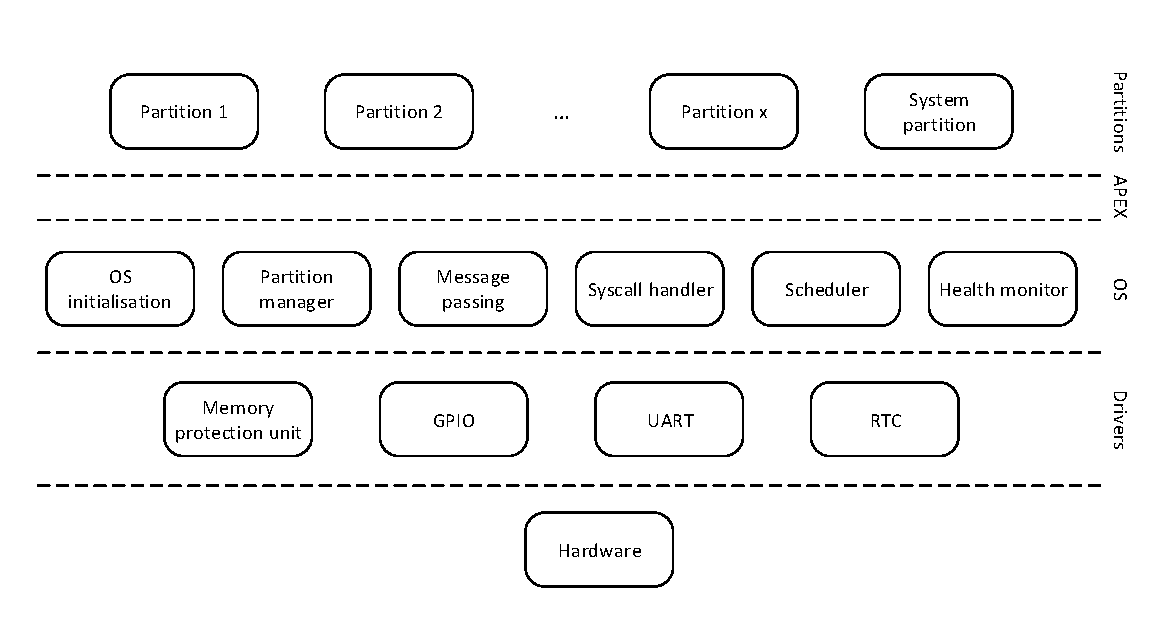
\includegraphics[width=\textwidth]{advanced_system_architecture.pdf}

\caption{An advanced system overview}
\label{fig:advanced_system}
\end{figure}

The following chapter will go through how all these components,
features and functionalities has been implemented.

